%%%%%%%%%%%%%%%%%%%%%%%%%%%%%%%%%%%%%%%%%
% Beamer Presentation
% LaTeX Template
% Version 1.0 (10/11/12)
%
% This template has been downloaded from:
% http://www.LaTeXTemplates.com
%
% License:
% CC BY-NC-SA 3.0 (http://creativecommons.org/licenses/by-nc-sa/3.0/)
%
%%%%%%%%%%%%%%%%%%%%%%%%%%%%%%%%%%%%%%%%%

%----------------------------------------------------------------------------------------
%	PACKAGES AND THEMES
%----------------------------------------------------------------------------------------

\documentclass{beamer}

\mode<presentation> {

% The Beamer class comes with a number of default slide themes
% which change the colors and layouts of slides. Below this is a list
% of all the themes, uncomment each in turn to see what they look like.

%\usetheme{default}
%\usetheme{AnnArbor}
%\usetheme{Antibes}
%\usetheme{Bergen}
%\usetheme{Berkeley}
%\usetheme{Berlin}
%\usetheme{Boadilla}
%\usetheme{CambridgeUS}
%\usetheme{Copenhagen}
%\usetheme{Darmstadt}
%\usetheme{Dresden}
%\usetheme{Frankfurt}
%\usetheme{Goettingen}
%\usetheme{Hannover}
%\usetheme{Ilmenau}
%\usetheme{JuanLesPins}
%\usetheme{Luebeck}
\usetheme{Madrid}
%\usetheme{Malmoe}
%\usetheme{Marburg}
%\usetheme{Montpellier}
%\usetheme{PaloAlto}
%\usetheme{Pittsburgh}
%\usetheme{Rochester}
%\usetheme{Singapore}
%\usetheme{Szeged}
%\usetheme{Warsaw}

% As well as themes, the Beamer class has a number of color themes
% for any slide theme. Uncomment each of these in turn to see how it
% changes the colors of your current slide theme.

%\usecolortheme{albatross}
%\usecolortheme{beaver}
%\usecolortheme{beetle}
%\usecolortheme{crane}
%\usecolortheme{dolphin}
%\usecolortheme{dove}
%\usecolortheme{fly}
%\usecolortheme{lily}
%\usecolortheme{orchid}
%\usecolortheme{rose}
%\usecolortheme{seagull}
%\usecolortheme{seahorse}
%\usecolortheme{whale}
%\usecolortheme{wolverine}

%\setbeamertemplate{footline} % To remove the footer line in all slides uncomment this line
%\setbeamertemplate{footline}[page number] % To replace the footer line in all slides with a simple slide count uncomment this line

%\setbeamertemplate{navigation symbols}{} % To remove the navigation symbols from the bottom of all slides uncomment this line
}

\usepackage{graphicx} % Allows including images
\usepackage{booktabs} % Allows the use of \toprule, \midrule and \bottomrule in tables
\usepackage{multirow}
\newcommand{\xmark}{\textcolor{red}{\text{\sffamily X}}}
\newcommand{\cmark}{\textcolor{green}{\checkmark}}
\newcommand{\tr}{\text{tr}}
\newcommand{\E}{\textbf{E}}
\newcommand{\diag}{\text{diag}}
\newcommand{\argmax}{\text{argmax}}
\newcommand{\argmin}{\text{argmin}}
\newcommand{\Cov}{\text{Cov}}
\newcommand{\Vol}{\text{Vol}}

%----------------------------------------------------------------------------------------
%	TITLE PAGE
%----------------------------------------------------------------------------------------


\title[Group talk]{The geometry of human perception: Inferring perception-induced metrics from fMRI data}

\author{Charles Zheng} % Your name
\institute[Stanford] % Your institution as it will appear on the bottom of every slide, may be shorthand to save space
{Stanford University}
\date{\today} % Date, can be changed to a custom date

\begin{document}

\begin{frame}
\titlepage % Print the title page as the first slide
(Joint work with Yuval Benjamini)
\end{frame}

\section{Introduction}

\begin{frame}
\frametitle{Similarity}
\begin{itemize}
\item You have an intuitive sense for whether two faces are 'similiar' or 'dissimilar'
\item Each person has their own \emph{similarity metric} for a given type of stimulus (e.g. faces, colors, etc.)
\item Take a particular type of stimulus, and suppose it lies in a space $\mathcal{X}$.  Your similarity metric is a function $d(x_1, x_2)$ for stimuli $x_1, x_2 \in \mathcal{X}$
\end{itemize}
\begin{center}
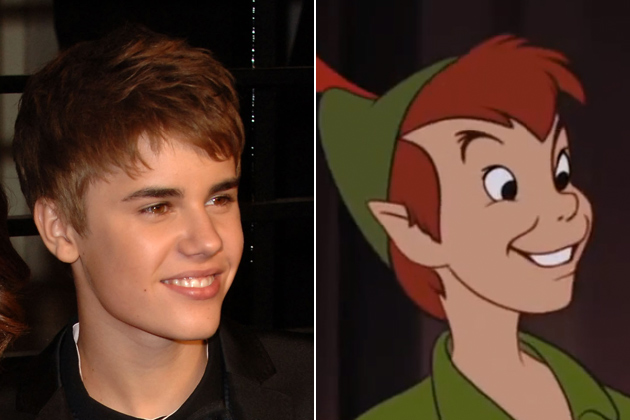
\includegraphics[scale = .12]{bieber.jpg}\hspace{1in}
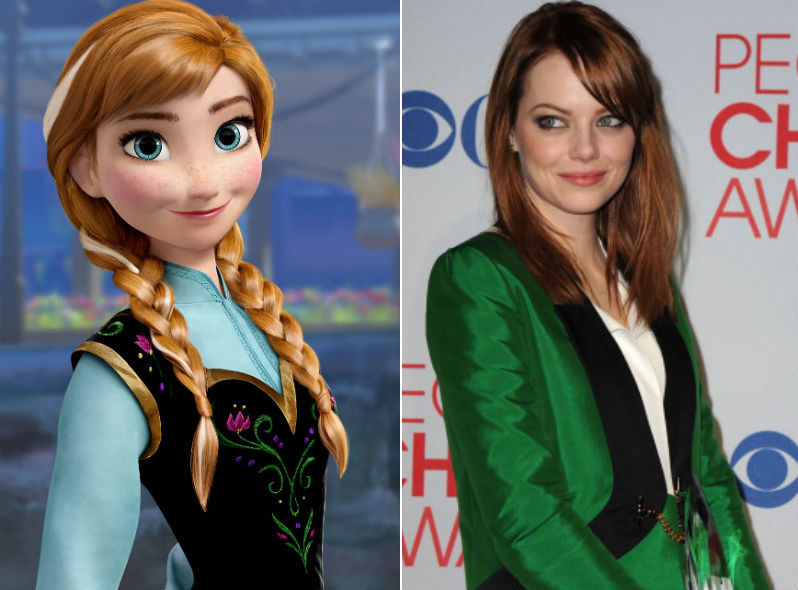
\includegraphics[scale = .12]{stone.jpg}
\end{center}
\[
d(\text{Bieber},\text{Peter Pan}) < d(\text{Bieber}, \text{Anna})
\]
\end{frame}

\begin{frame}
\frametitle{Perception-induced metric}
\begin{itemize}
\item Seeing (or hearing/smelling/touching) a stimulus triggers \emph{brain activity}.  The activity is random, but one can define a \emph{brain activity distribution} conditional on the triggering stimulus.
\item Let $X \in \mathcal{X}$ be a random stimulus, let $Y \in \mathcal{Y}$ be your brain activity.  Define $F_x$ to be the conditional distribution of $Y|X=x$.
\item Working assumption: your intuitive similarity metric $d(x_1,x_2)$ is related to the \emph{perception-induced metric} $d_\iota$ defined by
\[
d_\iota(x_1,x_2) = D(F_{x_1}, F_{x_2})
\]
for some distance metric $D$ on probability measures.
\end{itemize}
\begin{center}
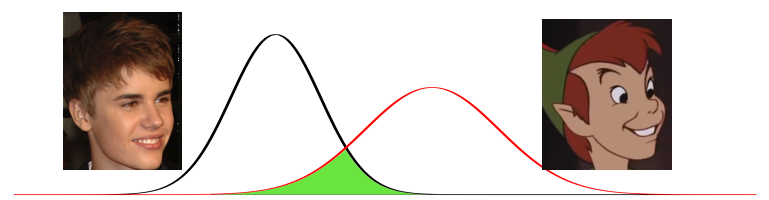
\includegraphics[scale = .12]{similarity.png}
\end{center}
\end{frame}

\begin{frame}
\frametitle{Functional MRI allows us to infer the metric}
\begin{itemize}
\item In fMRI, one records the subject's response $y_i$ to a stimulus $x_i$,
for $i = 1,\hdots, n$ (e.g. $n = 3000$)
\item The recorded $y_i$ is actually a 'filtered' version of the brain activity (some information is lost)
\item By fitting a model to the data, one can estimate the conditional distribution of $Y|x$ and hence estimate the perception-induced metric $d_\iota$.
\end{itemize}
\begin{center}
\begin{tabular}{ccc}
\hline
Stimuli & & Response\\ \hline
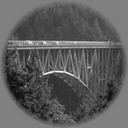
\includegraphics[scale = .3]{img1.png} & \hspace{1in} & 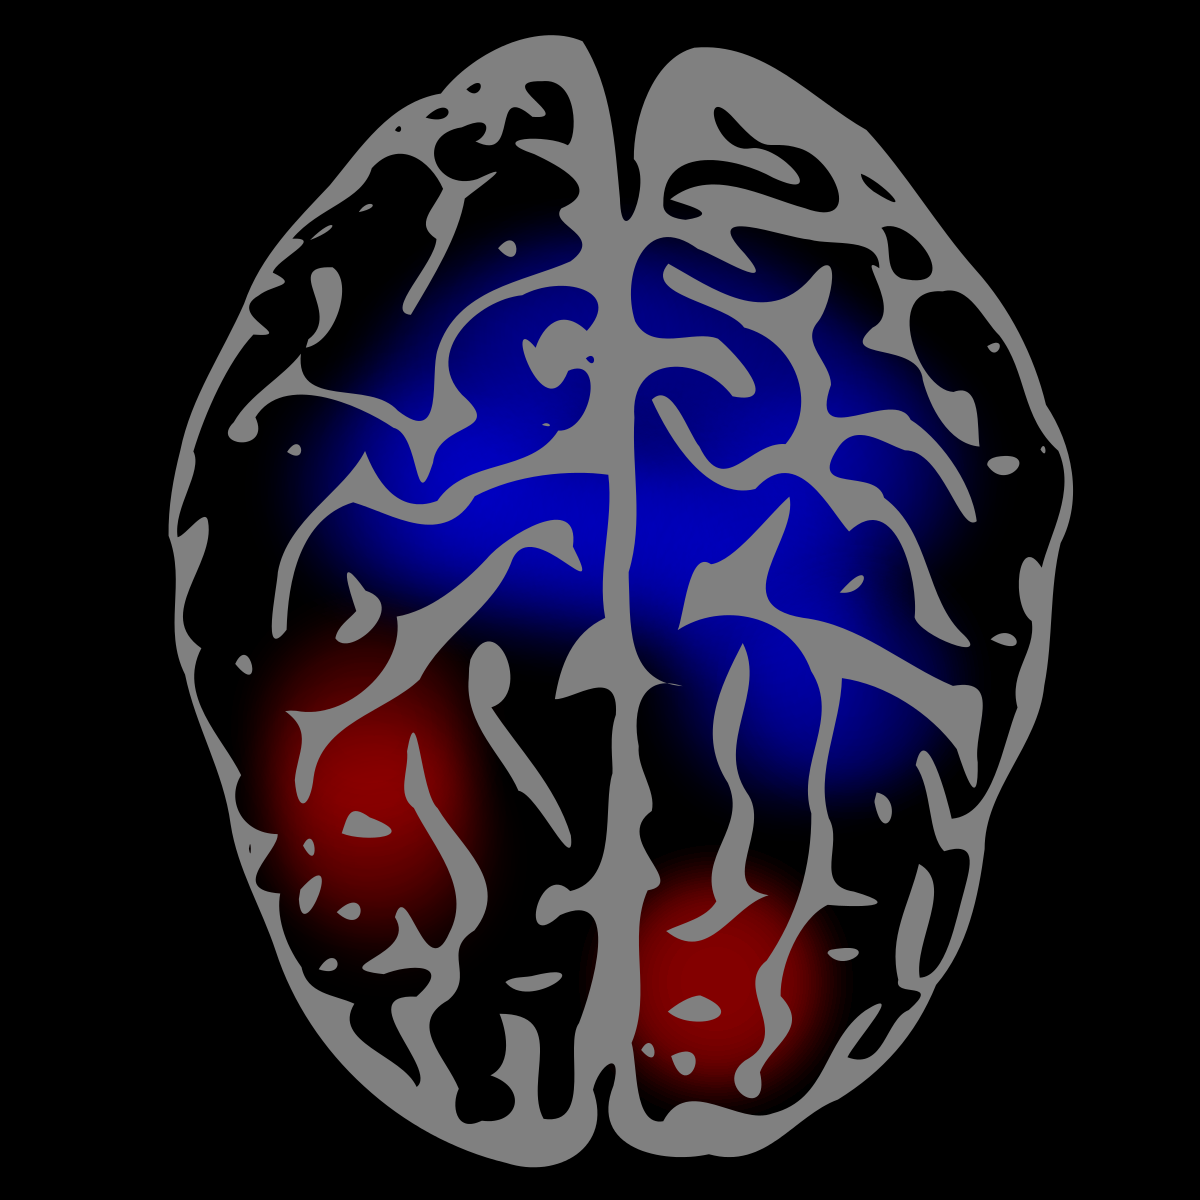
\includegraphics[scale = 0.035]{brain1.png} \\ \hline
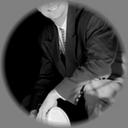
\includegraphics[scale = .3]{img2.png} & \hspace{1in} & 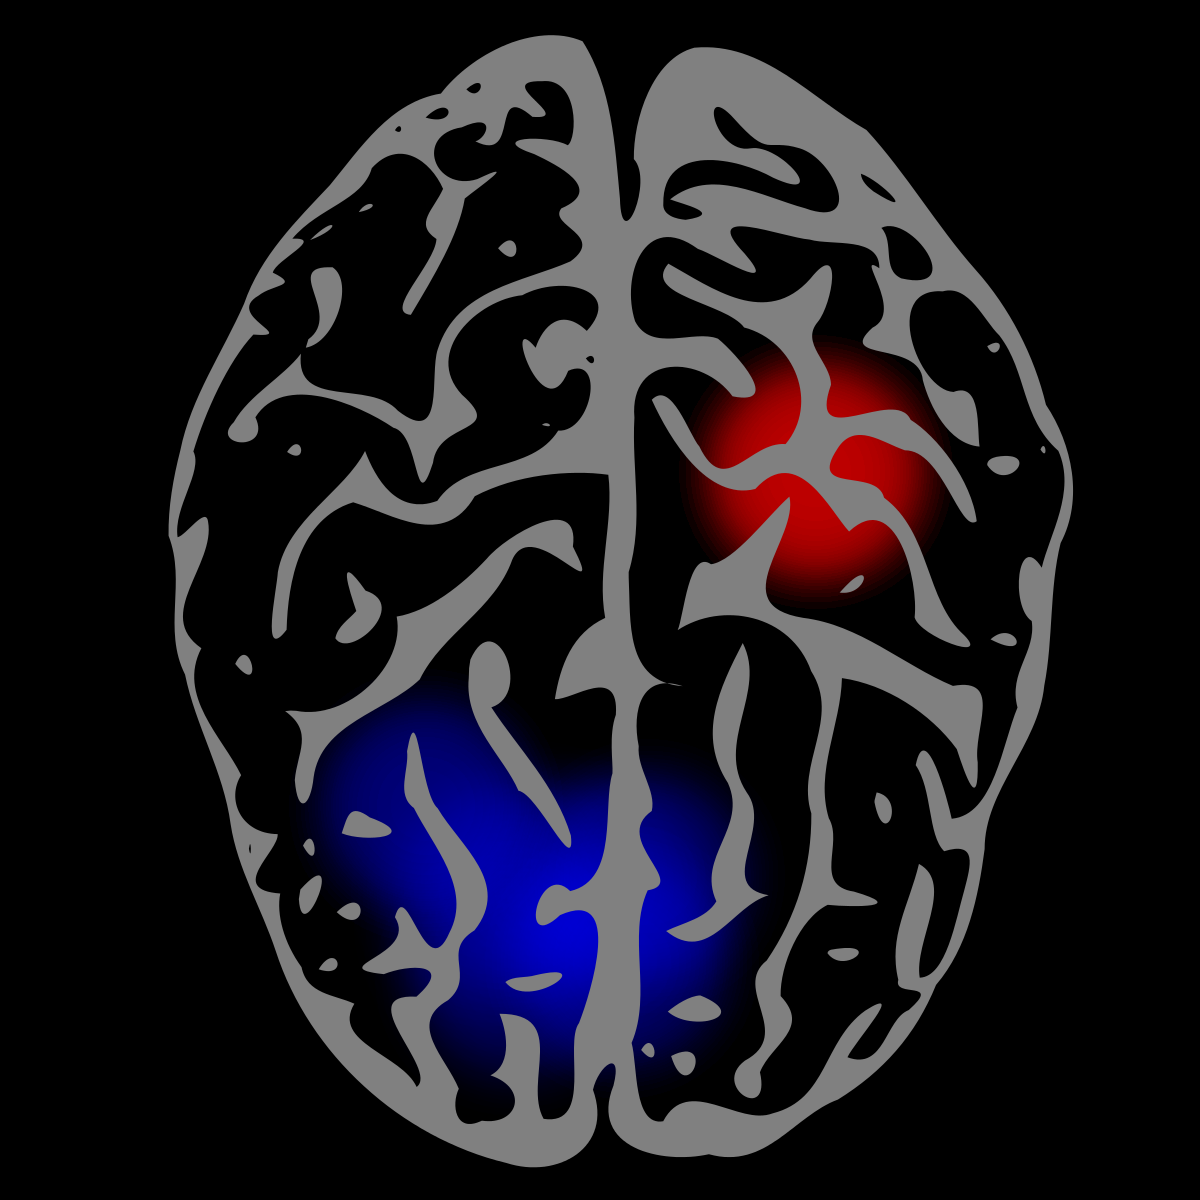
\includegraphics[scale = 0.035]{brain2.png} \\ \hline
\hspace{1in} & \hspace{1in} & \hspace{1in}
\end{tabular}
\end{center}
\end{frame}

\begin{frame}
\frametitle{References}
\begin{itemize}
\item Kay, KN., Naselaris, T., Prenger, R. J., and Gallant, J. L.
  ``Identifying natural images from human brain
  activity''. \emph{Nature} (2008)
\item Naselaris, et al. ``Bayesian reconstruction of natural images
  from human brain activity''.  \emph{Neuron} (2009)
\item Vu, V. Q., Ravikumar, P., Naselaris, T., Kay, K. N., and Yu, B.
  ``Encoding and decoding V1 fMRI responses to natural images with
  sparse nonparametric models'', \emph{The Annals of Applied
    Statistics}. (2011)
\item Chen, M., Han, J,. Hu, X., Jiang, Xi., Guo, L. and Liu, T.
  ``Survey of encoding and decoding of visual stimulus via fMRI: an
  image analysis perspective.'' \emph{Brain Imaging and
    Behavior}. (2014)
\end{itemize}
\end{frame}

\end{document}












